%!TEX root = top.tex
\section{Related Work}
Our model draws success from several areas, including deep networks, multi-scale features for semantic segmentation, and attention models.

%\paragraph{Deep networks} 
\textbf{Deep networks:} Deep Convolutional Neural Networks (DCNNs) \cite{lecun1998gradient} have demonstrated state-of-the-art performance on several computer vision tasks, including image classification \cite{krizhevsky2012imagenet, sermanet2013overfeat, szegedy2014going, simonyan2014very, papandreou2014untangling} and object detection \cite{girshick2014rich, he2014spatial}. For the semantic image segmentation task, state-of-the-art methods are variants of the fully convolutional
neural networks (FCNs) \cite{long2014fully}, including \cite{chen2014semantic, dai2015boxsup, lin2015efficient, noh2015learning, zheng2015conditional}. In particular, our method builds upon the current state-of-the-art DeepLab model \cite{chen2014semantic}. %, which employs {\`a} trous algorithm \cite{Mall99} and has faster training time.

\begin{figure}    
  \centering
  \addtolength{\tabcolsep}{-5pt}
  \begin{tabular}{cc}
   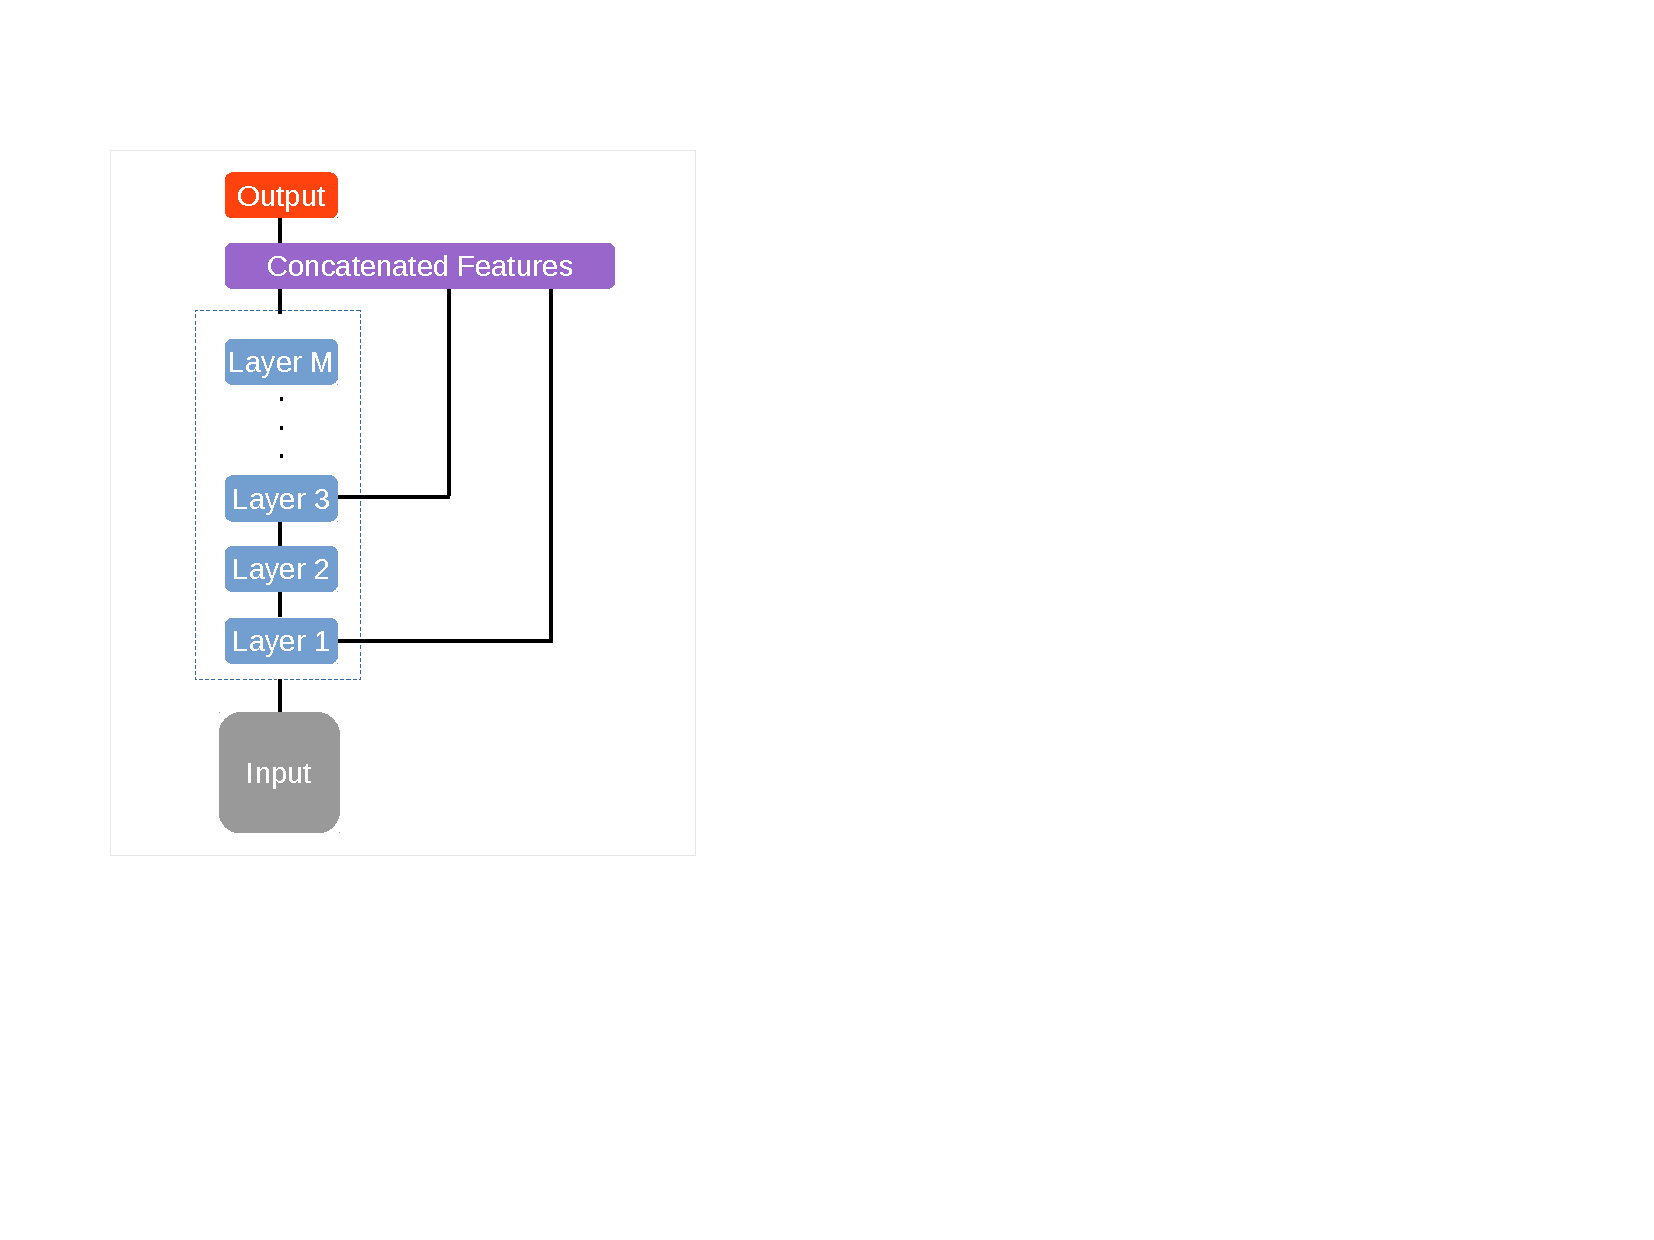
\includegraphics[height=0.59\linewidth]{fig/skip_net3.pdf} &
   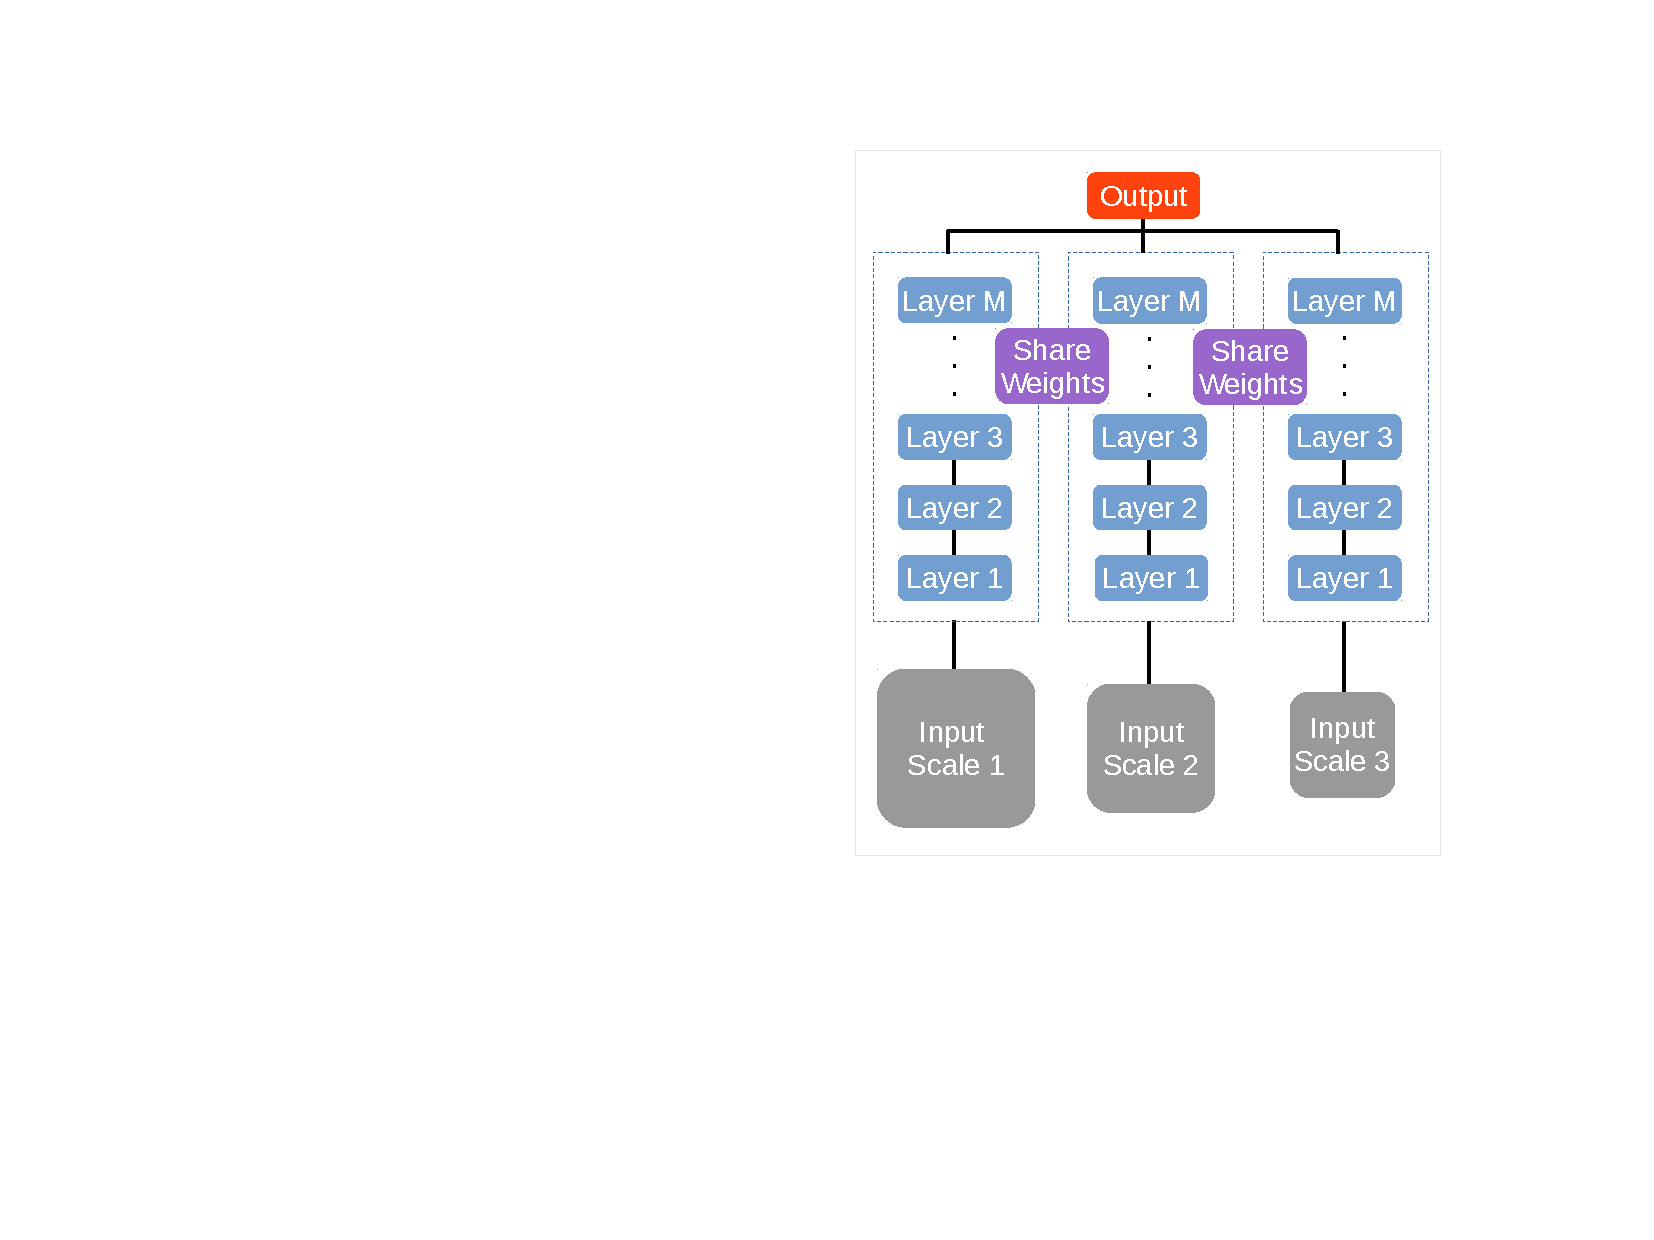
\includegraphics[height=0.59\linewidth]{fig/share_net3.pdf} \\
   (a) skip-net &
   (b) share-net \\
  \end{tabular}
  \vspace{1pt}
  \caption{Different network structures for extracting multi-scale features: (a) Skip-net: features from intermediate layers are fused to produce the final output. (b) Share-net: multi-scale inputs are applied to a shared network for prediction. In this work, we demonstrate the effectiveness of the share-net when combined with attention mechanisms over scales.}
  \label{fig:nets}
\end{figure}  

%\paragraph{Multi-scale features} 
\textbf{Multi-scale features:} It is known that multi-scale features are useful for computer vision tasks, \eg, \cite{florack1996gaussian, arbelaez2011contour}. %weber1995robust
In the context of deep networks for semantic segmentation, we mainly discuss two types of networks that exploit multi-scale features. The first type, {\it skip-net}, exploits features from different levels of the network. For example, FCN-8s \cite{long2014fully} gradually learns finer-scale prediction from lower layers (initialized with coarser-scale prediction). Hariharan \etal \cite{hariharan2014hypercolumns} classified a pixel with hypercolumn representation (\ie, concatenation of
features from intermediate layers). Mostajabi \etal \cite{mostajabi2014feedforward} classified a superpixel with features extracted at zoom-out spatial levels from a small proximal neighborhood to the whole image region. DeepLab-MSc (DeepLab with Multi-Scale features) \cite{chen2014semantic} applied Multi-Layer Perceptrons (MLPs) to the input image and to the outputs of pooling layers, in order to extract multi-scale features. ParseNet \cite{liu2015parsenet} aggregated features over the whole image to provide global contextual information. 

The second type, {\it share-net}, applies multi-scale input images to a shared network. For example, Farabet \etal \cite{farabet2013learning} employed a Laplacian pyramid, passed each scale through a shared network, and fused the features from all the scales. Lin \etal \cite{lin2015efficient} resized the input image for three scales and concatenated the resulting three-scale features to generate the unary and pairwise potentials of a Conditional Random Field (CRF). Pinheiro \etal
\cite{pinheiro2013recurrent}, instead of applying multi-scale input images at once, fed multi-scale images at different stages in a recurrent convolutional neural network. This share-net strategy has also been employed during the test stage for a better performance by Dai \etal \cite{dai2015boxsup}. In this work, we extend DeepLab \cite{chen2014semantic} to be a type of {\it share-net} and demonstrate its effectiveness on three challenging datasets. Note that Eigen and Fergus
\cite{eigen2014predicting} fed input images to DCNNs at three scales from coarse to fine sequentially. The DCNNs at different scales have different structures, and a two-step training process is required for their model.

%\paragraph{Attention models for deep network} 
\textbf{Attention models for deep networks:} In computer vision, attention models have been used widely used for image classification \cite{cao2015look, gregor2015draw, xiao2015application} and object detection \cite{ba2014multiple, caicedo2015active, yoo2015attentionnet}. Mnih \etal \cite{mnih2014recurrent} learn an attention model that adaptively selects image regions for processing. However, their attention model is not differentiable, which is necessary for standard backpropagation during training. On the other hand, Gregor \etal \cite{gregor2015draw} employ a differentiable attention model to specify where to read/write image regions for image generation. 

Bahdanau \etal \cite{bahdanau2014neural} propose an attention model that softly weights the importance of input words in a source sentence when predicting a target word for machine translation. Following this, Xu \etal \cite{xu2015show} and Yao \etal \cite{yao2015describing} use attention models for image captioning and video captioning respectively. These methods apply attention in the 2D spatial and/or temporal dimension while we use attention to identify the most relevant scales. 

%\paragraph{Attention to scales} 
\textbf{Attention to scale:} To merge the predictions from multi-scale features, there are two common approachs: average-pooling \cite{ciresan2012multi, dai2015boxsup} or max-pooling \cite{felzenszwalb2010object, papandreou2014untangling} over scales. Motivated by \cite{bahdanau2014neural}, we propose to jointly learn an attention model that softly weights the features from different input scales when predicting the semantic label of a pixel. The final output of our model is produced by the
weighted sum of score maps across all the scales. We show that the proposed attention model not only improves performance over average- and max-pooling, but also allows us to diagnostically {\it visualize} the importance of features at different positions and scales, separating us from existing work that exploits multi-scale features for semantic segmentation.
